
If a matrix style display is used with a microcontroller, there are a lot of different ways to draw graphical elements. This section covers only the ways used in this project. 

\subsubsection{Matrix displays}
Since most displays produced have a rectangular shape, the amount of pixel they hold is calculated like the surface of an rectangular. The number of pixels on both axis are multiplied and we get the total amount of pixels we have to manipulate. So it is obvious that the memory size of a picture explodes with its resolution. A display with a size of $1200 \times 825$ pixels and a colour depth of 24 bit serves as an example. This resolution results in amount of $1200\cdot825=990'000$ pixels and thus $1200\cdot825\cdot24=23'760'000$ bits. This is a huge amount of data to process with a standard microcontroller.
To handle the data transfer between memory and display, special parallel driver chips are used. These drivers are mapping the right memory location to the desired pixel on the display. More expensive driver chips have built in memory. To access it from a host \acs{cpu}, parallel or serial bus interfaces are used. If a display is rectangular, the information with the pixel value can be ordered in a matrix.
A good option to store an image is therefore an array.
The advantage of an array is the easy access and the memory allocation given in various programming languages.
In C for example, memory of an array has to be allocated at consecutive addresses \cite{ISO/IEC9899}.
 
% \begin{align}
%n = \lfloor \log_{2}(176) \rfloor = 8 bit.
% \end{align}

% bit.   

%\begin{figure}[H]
%	\centering
%	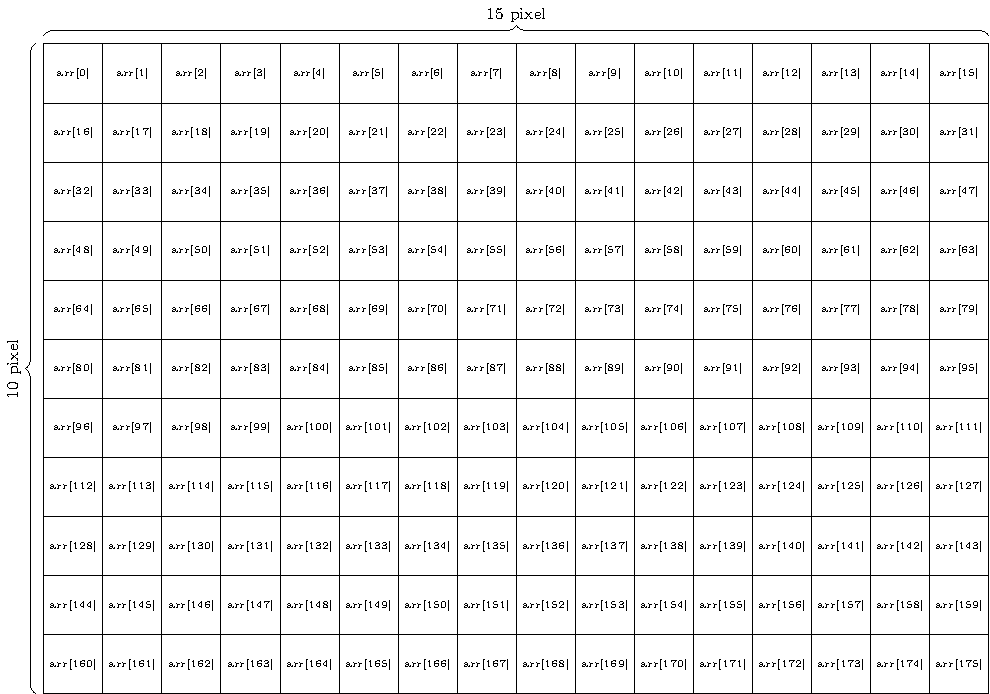
\includegraphics[width=1\textwidth]{2-theory/drawing-graphics/graphics/matrix.pdf}
%	\caption{$16\times 11$ pixel display with a flat matrix \label{theory:matrix}}
%\end{figure}

% \begin{align}
%n = \lfloor \log_{2}(11) \rfloor + \lfloor\rfloor\log_{2}(16) \rfloor = 8 bit.
%\end{align}

%\begin{figure}[H]
%	\centering
%	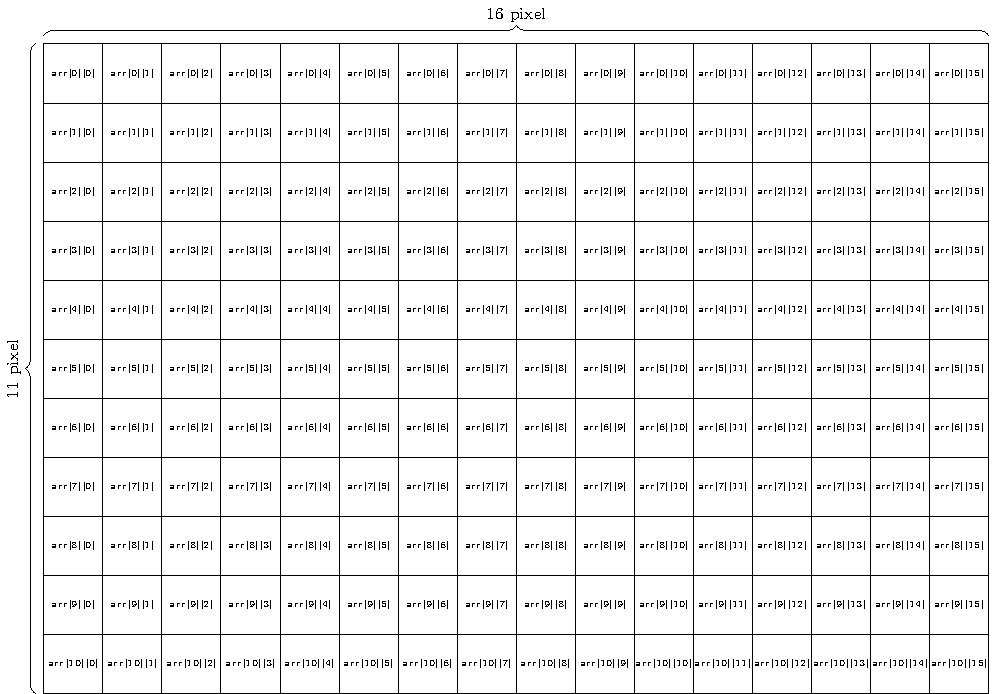
\includegraphics[width=1\textwidth]{2-theory/drawing-graphics/graphics/matrix2.pdf}
%	\caption{$16\times 11$ display with a two dimensional matrix\label{theory:matrix2}}
%\end{figure}

\subsubsection{Double buffering}
To write an image to a display, two separate memory accesses are carried out.
The first writes the image into the buffer, the second takes this data and displays on screen.
By using two buffers, it is possible to accelerate this process.
This is shown in Figure \ref{theory:buffer}.

\begin{figure}[ht]
	\centering
	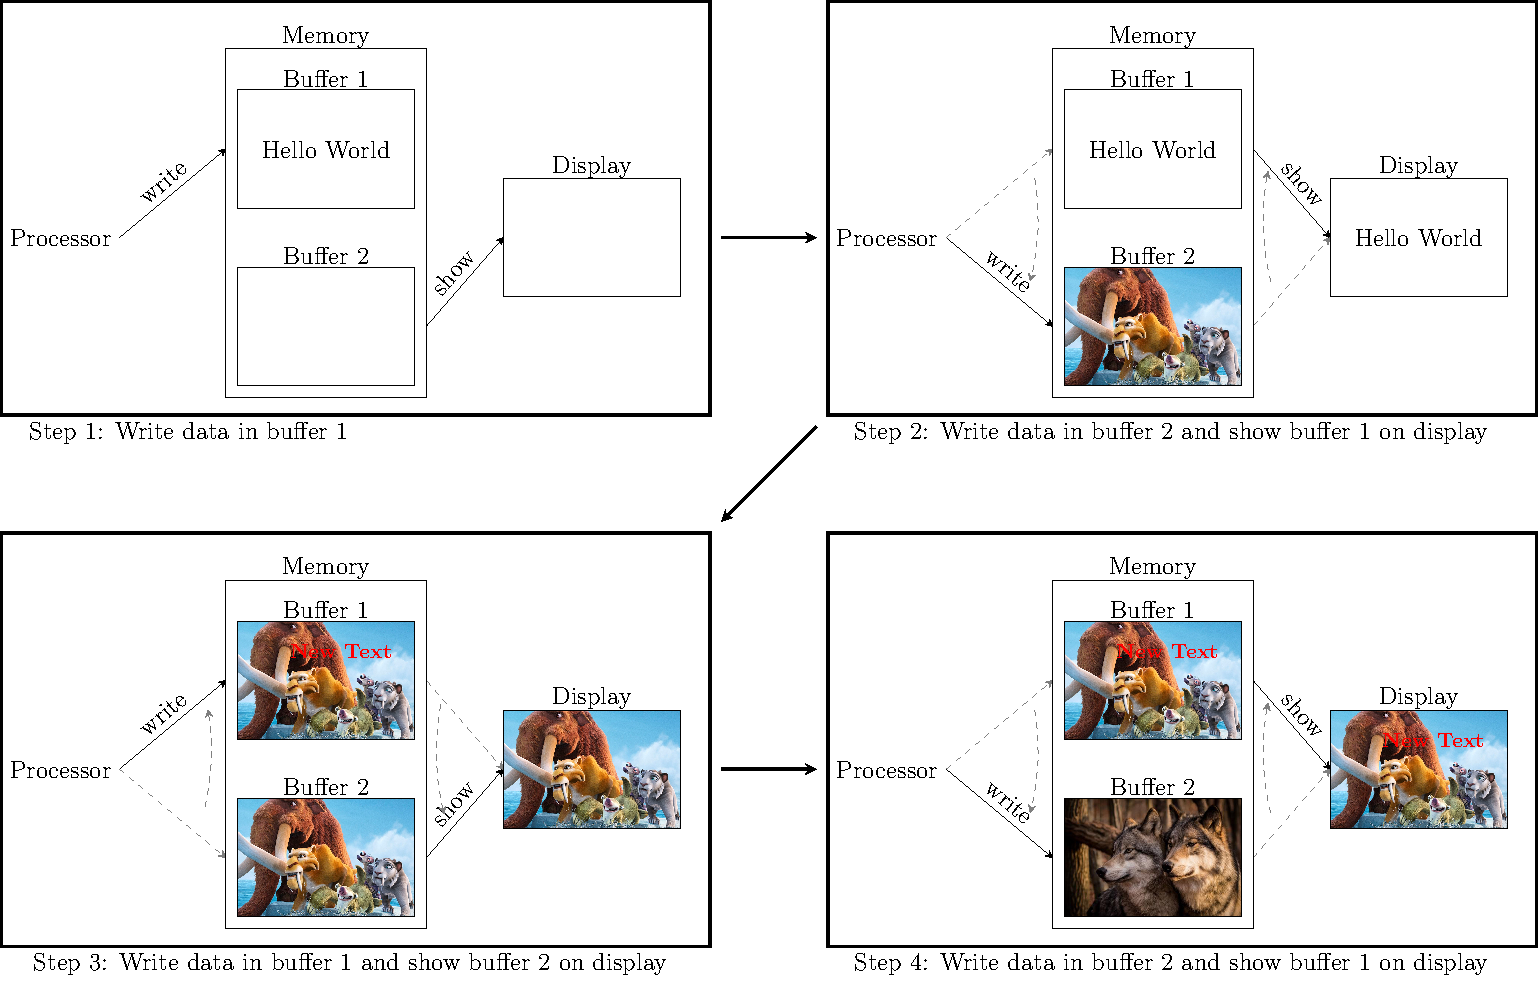
\includegraphics[width=0.9\textwidth]{2-theory/drawing-graphics/graphics/buffer.pdf}
	\caption{Double buffering.\label{theory:buffer}}
\end{figure}

While the new data is written in to one buffer, the screen displays the data located in the other buffer at the same time.

\subsubsection{Compressed fonts}\label{theory:CompressedFonts}
To write a specific character to the display, the controller needs to know how the font is structured.
Figure \ref{theory:font12} shows how the character A could look.
\begin{figure}[ht]
	\centering
	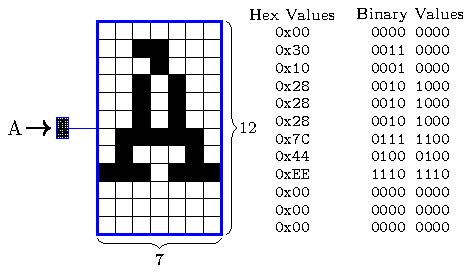
\includegraphics[width=0.8\textwidth]{2-theory/drawing-graphics/graphics/font12.pdf}
	\caption{Creation of a simple seven to twelve pixel sized font.\label{theory:font12}}
\end{figure}
The character is stored this way into the memory and can be accessed just like a look-up table.
If fonts are stored with a $12\times 7$ pixel mask, every character occupies 12 bytes memory.

To display characters in color, 8 more bits for the color depth are needed.
this is visualized in Figure \ref{fig:ganzes_fig}. During the mapping of the font mask to the buffer memory the desired colour value is chosen and put in every place the mask has a set pixel. With using this method save fonts and writing characters in a buffer instead of using the full depth is the font size multiplied with the colour depth.  

\begin{figure}[ht]
	\centering
	\subfigure[1 bit colour font\label{fig:1bitcolor}]{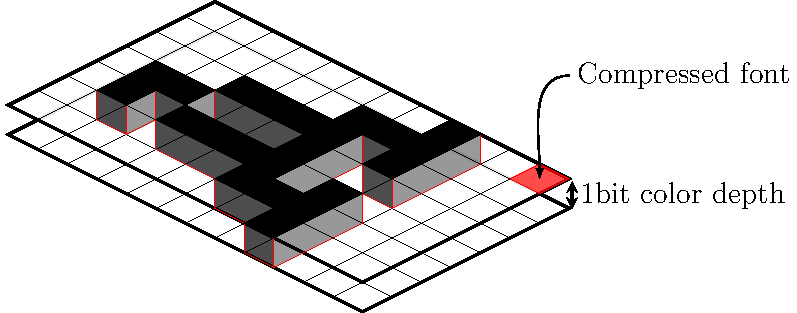
\includegraphics[width=0.49\linewidth]{2-theory/drawing-graphics/graphics/drawingfont.pdf}}
	\subfigure[8 bit colour font (value for blue)\label{fig:Colorblue}]{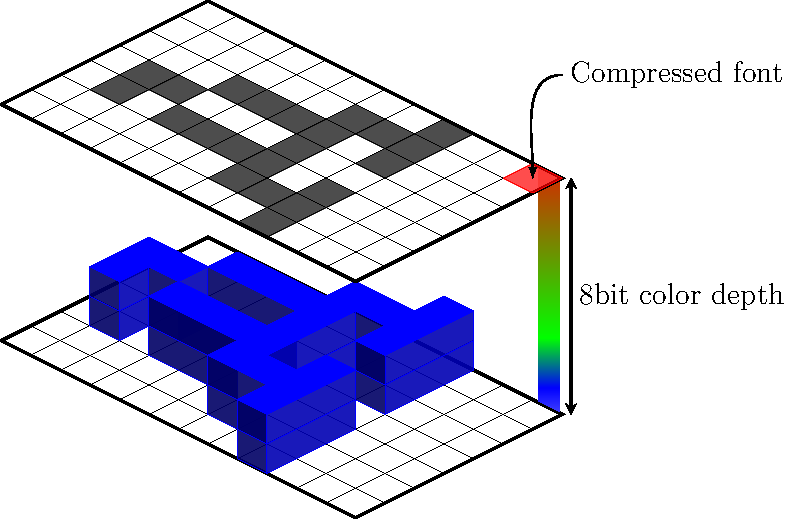
\includegraphics[width=0.49\linewidth]{2-theory/drawing-graphics/graphics/drawingfont8blue.pdf}}
	\subfigure[8 bit colour font (value for green) \label{fig:Colorgreen}]{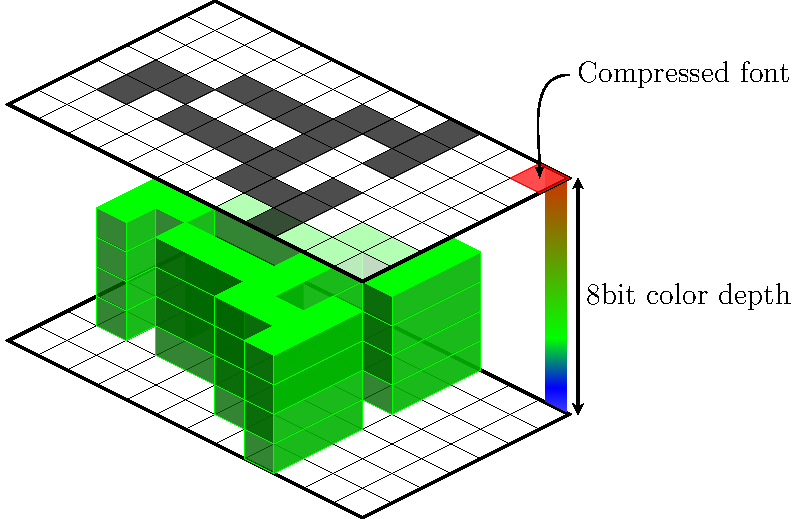
\includegraphics[width=0.49\linewidth]{2-theory/drawing-graphics/graphics/drawingfont8green.pdf}}
	\subfigure[8 bit colour font (value for red) \label{fig:Colorred}]{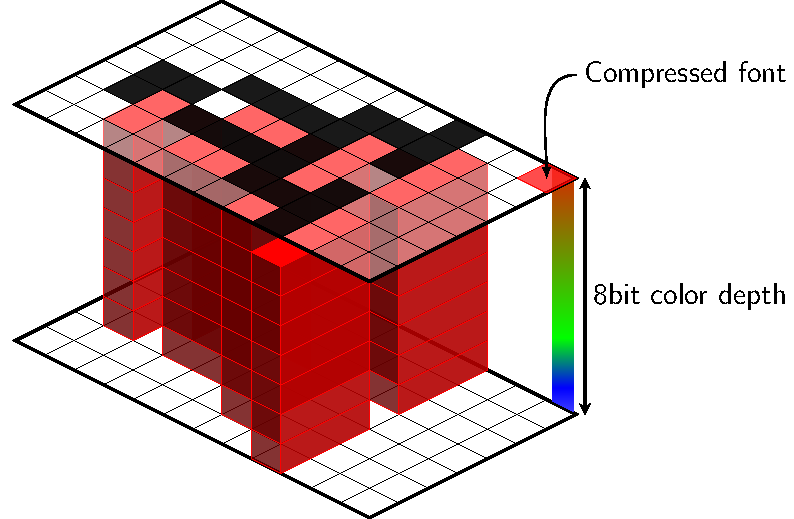
\includegraphics[width=0.49\linewidth]{2-theory/drawing-graphics/graphics/drawingfont8red.pdf}}
	\caption{$12 \times 7$ pixel font mask displayed with $1$- and $8$bit colour depth}
	\label{fig:ganzes_fig}
\end{figure}



